
\section{Test cases}

\subsection{Verification of basic MGM implementation}
The first step of my test series was to verify the basic correctness of my implementation of the MGM methodology. For this purpose I started from the requirement that for a single mesh case MGM (as an unstructured solver) should yield exactly the same solution as UGLMAT or USCARC.

In fact, I could actually prove this for many different single mesh test cases, so that I no longer doubt the correct calculation and assignment of Neumann boundary values along inner obstructions.



\subsection{Comparison of different boundary conditions along $\partial M$}
My next step was to compare UGLMAT and USCARC versus MGM for different multi-mesh cases. 
As boundary values along $\partial M$ I tested the 'Simple mean value (SM)' and the 'Linear Extrapolation (LE)'. The Taylor-variant is in development, but not yet finished.

The (LE) variant was worth a test from my point of view, because it as relatively easy to implement and storing the additionally needed interface values from the second last step '${n-2}$' does not require much space. 

\subsubsection{Case 1}
Let's start with a very simple test with only one obstruction which is completely contained in one mesh. 
\begin{figure}[H]
\begin{center}
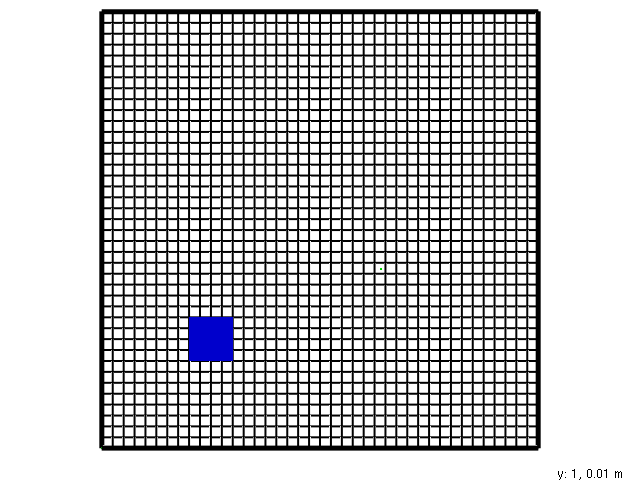
\includegraphics[width=7cm]{\figPath/b1_s0002.png}
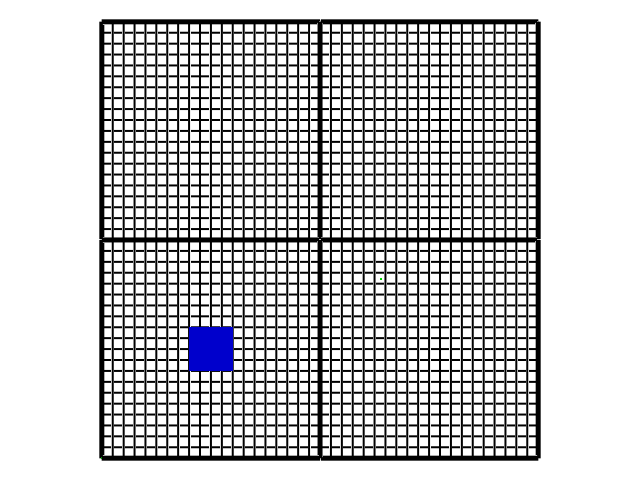
\includegraphics[width=7cm]{\figPath/b4_le_s0002.png}
\end{center}
\caption{Case 1}
\label{FIG_MGM_Grid}
\end{figure}
\newpage
Then the simple mean value (SM) gives

\begin{figure}[H]
\begin{center}
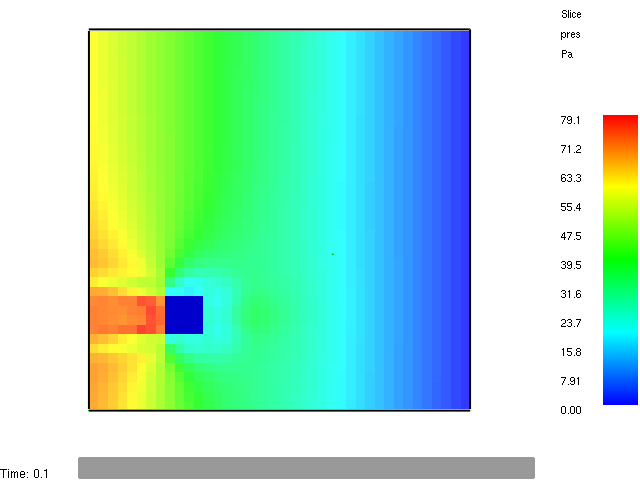
\includegraphics[width=8cm]{\figPath/b1_0062.png}
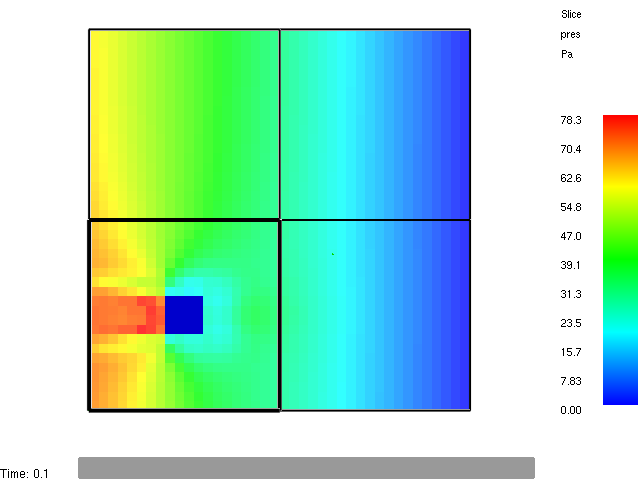
\includegraphics[width=8cm]{\figPath/b4_sm_0062.png}
\end{center}
\caption{Simple mean value  (SM) for Case 1}
\label{FIG_MGM_Grid}
\end{figure}


and the linear extrapolation setting (LE) gives

\begin{figure}[H]
\begin{center}
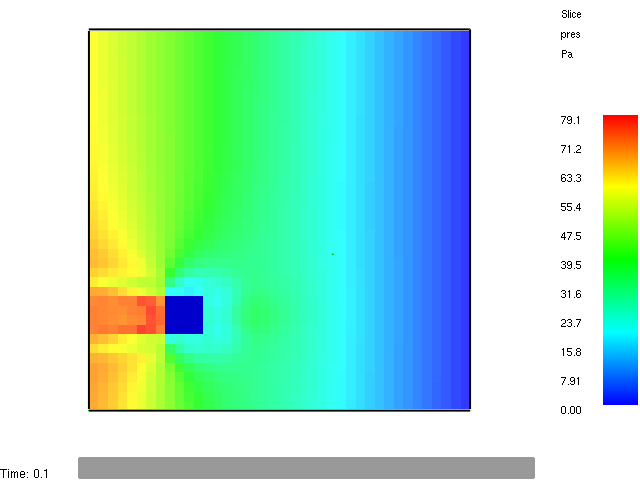
\includegraphics[width=8cm]{\figPath/b1_0062.png}
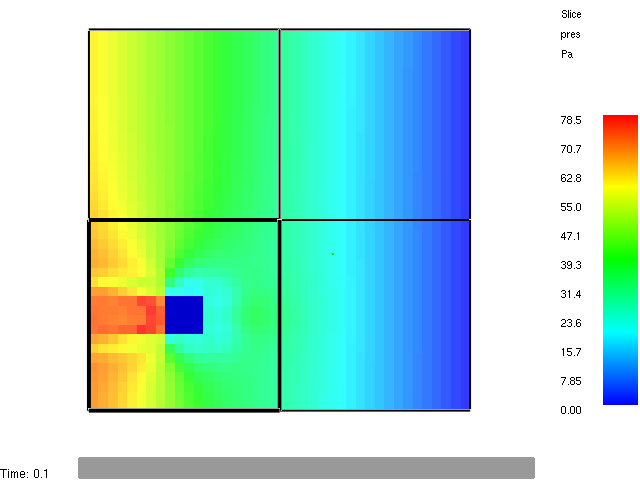
\includegraphics[width=8 cm]{\figPath/b4_le_0062.png}
\end{center}
\caption{Linear extrapolation  (LE) for Case 1}
\label{FIG_MGM_Grid}
\end{figure}


These both seems to be very similar.  But please note the displayed ranges (they are unchanged, as originally displayed by smokeview).
The display range for (LE) is a little closer to the single-mesh range. But I don't know if this matters.

\newpage
\subsubsection{Dancing\_eddies}
The usual pressure history plots for UGLMAT and USCARC (which both provide the same) against MGM with the (SM) and (LE) boundary settings.
\begin{figure}[H]
\begin{center}
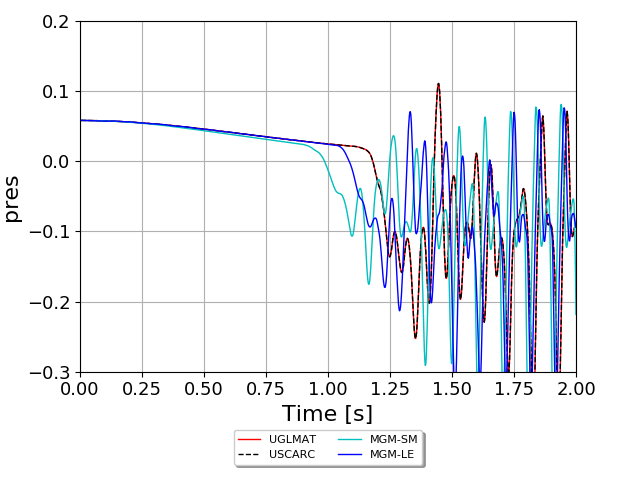
\includegraphics[width=10cm]{\figPath/dancing_eddies_pres.png}
\end{center}
\caption{Pressure histories of UGLMAT, USCARC, MGM-SM and MGM-LE for dancing\_eddies}
\label{FIG_MGM_de}
\end{figure}

And a more zoomed view here
\begin{figure}[H]
\begin{center}
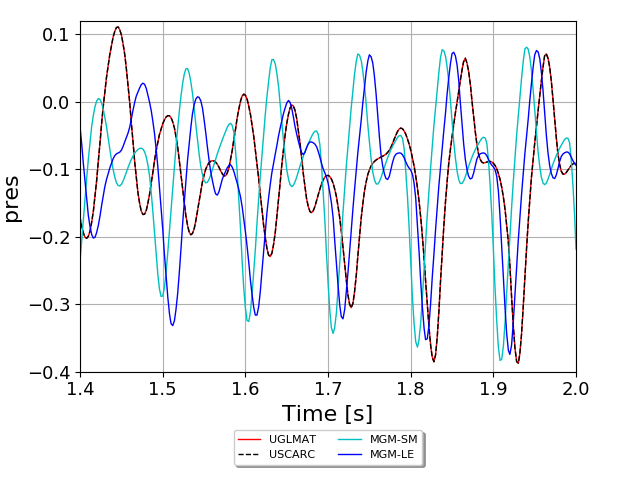
\includegraphics[width=10cm]{\figPath/dancing_eddies_pres2.png}
\end{center}
\caption{Zoomed pressure histories of UGLMAT, USCARC, MGM-SM and MGM-LE for dancing\_eddies}
\label{FIG_MGM_de}
\end{figure}

Here the differences seem to be more pronounced with a slight advantage for the linear extrapolation (the blue one). But they both don't fit the course of the
really unstructured solutions.

\newpage
\subsubsection{Pressure\_Iteration3d}
This is my pressure\_iteration3d case from the Pressure\_Solver directory (different and steadily changing ramp-based inflows from xmin, ymin and zmin)
with the pressure history for the green device position.

\begin{figure}[H]
\begin{center}
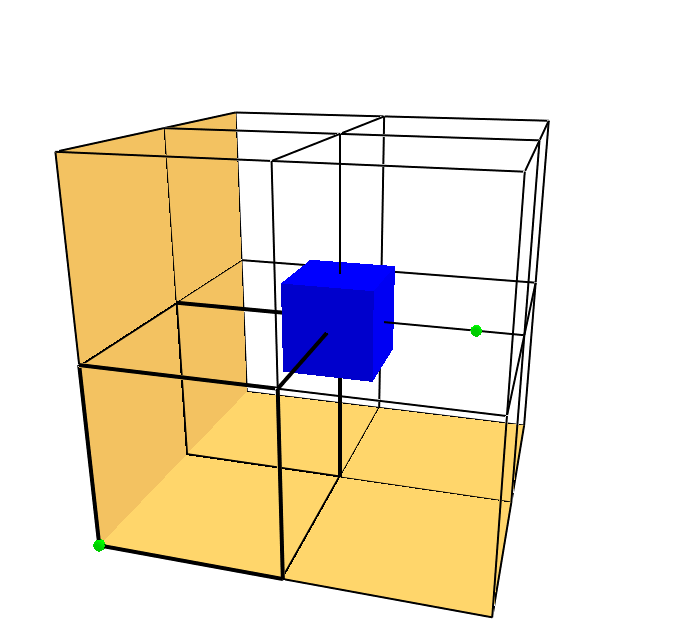
\includegraphics[width=5cm]{\figPath/pressure_iteration3d_uscarc_s0000.png}
\end{center}
\caption{pressure\_iteration3d case}
\label{FIG_MGM_pi}
\end{figure}

And here again are the plots for UGLMAT and USCARC (which again both provide the same) against MGM with the (SM) and (LE) boundary settings.
\begin{figure}[H]
\begin{center}
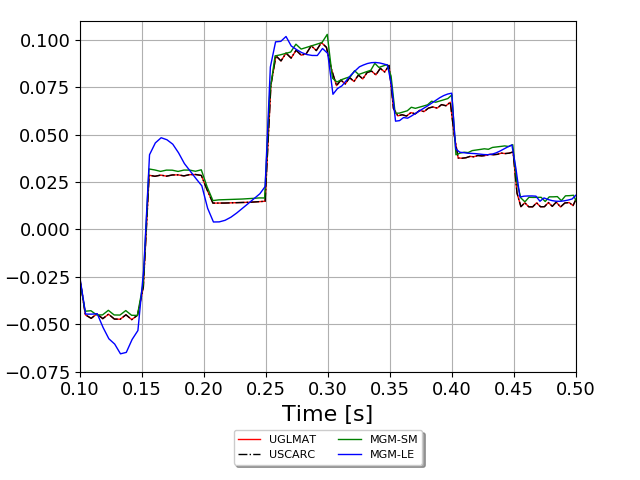
\includegraphics[width=12cm]{\figPath/pressure_iteration3d_pres.png}
\end{center}
\caption{Pressure histories of UGLMAT, USCARC, MGM-SM and MGM-LE for pressure\_iteration3d}
\label{FIG_MGM_pi}
\end{figure}

Here, the simple (SM) boundary condition seems to do the better job. But due to the steadily changing inflow conditions in this case this might be an issue of bad initial values for the extrapolation. 



